\title{Welcome to Informatica Intelligent Cloud Services}


\author{Sandeep Khandelwal}
\affiliation{%
  \institution{Indiana University}
  \city{Bloomington} 
  \state{IN} 
  \postcode{47408}
  \country{USA}
}
\email{skhande@iu.edu}

% The default list of authors is too long for headers}
\renewcommand{\shortauthors}{S. Khandelwal}


\begin{abstract}
	
There is massive amount of on-premise and cloud-based data. In today's world data has different format (structured data, semi-structured and unstructured data), volume (data size is upto hundreds of terabytes) and velocity (amount of data getting generated per second is too huge). Every organization has a necessity to integrate such kind of data between on-premise and cloud-based systems. Informatica Intelligent Cloud Services (IICS) provide complete suite of integration for such kind of diverse and unique requirement.

\end{abstract}

\keywords{hid-sp18-511, IICS, Informatica, ETL, Data Integration}


\maketitle


\section{Introduction}

Informatica Intelligent Cloud Services is built on micro service architecture and provide 
capability of data integration between cloud-based and on-premise systems. IICS~\cite{hid-sp18-511-iics} provide integration capability in four areas mainly Integration Cloud, Data Quality & Governance Cloud, Master Data Management Cloud, and Data Security Cloud (IICS)~\cite{hid-sp18-511-iics}. 

\section{Figures}

In Figure~\ref{f:fly} see the wide area of Informatica Integration Cloud Services (IICS)~\cite{hid-sp18-511-iics}.

\begin{figure}[!ht]
  \centering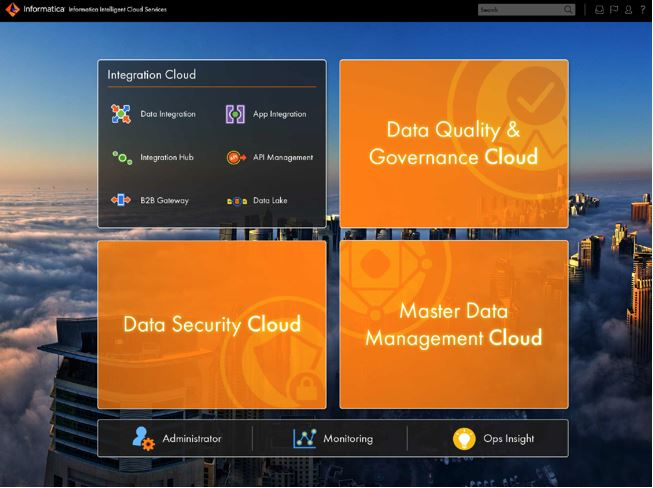
\includegraphics[width=\columnwidth]{images/IICS-0.jpg}
  \caption{IICS}\label{f:fly}
\end{figure}

To avoid copying the example figure in each hid directory, we actually
import it from the hid-sample directory. Lets assume you have a figure
in the image directory called myfigure.pdf. You can than replace the
line in the example with

\begin{verbatim}
\centering\includegraphics[width=\columnwidth]{images/myfigure.pdf}
\end{verbatim}

In case you use png than you must have a png that is at least 300dpi
(find out what that means and how to do that) and use 

\begin{verbatim}
\centering\includegraphics[width=\columnwidth]{images/myotehrfigure.png}
\end{verbatim}

When modifying the example, please do not check in the images from the
examples into your images directory as you will not need them for your
paper. Instead use images that you like to include. If you do not have
any images, do not palce anything in the images folder. However most
technologies could benefit for one image. Make sure you do not
plagiarize the image. Find out from the hand book how to do that. Any
plagiarism of images will result that we return the paper without
review as you have not understood how plagiarism works.

\section{Tables}

In case you need to create tables, you can do this with online tools
(if you do not mind sharing your data) such as
\url{https://www.tablesgenerator.com/} or other such tools (please
google for them). They even allow you to manage tables as CSV.

or generate them by hand while using the provided template in Table
\ref{t:mytable}. Note that
the caption is before the tabular environment.

\begin{table}[htb]
\centering
\caption{My caption}
\label{t:mytabble}
\begin{tabular}{lll}
1 & 2 & 3 \\
\toprule
4 & 5 & 6 \\
7 & 8 & 9
\end{tabular}
\end{table}

\section{Quotes}

Do not use double quotes \verb|"| but use \LaTeX\ ``quotes''. Quotes
{\bf MUST} not be used to highlight works. Quotes are {\bf STRICTLY}
used for quoting text from sources with citation following. If we find
a quote that is not followed by a citation we will return the paper
without review.

\section{Labels}

Do not use actual numbers in the taxt after you write for example
Figure 1 use the ref for the figure while using its label. In our
example it is Figure~\ref{f:fly} and Table Figure~\ref{t:mytabble}.
See the source for the example.

\section{Footnotes}

Footnotes must be avoided in papers. All URLs must be included as full
references and citations and used with the \verb|\cite| command
\footnote{do not use footnotes}. You {\bf must} not use urls in the
text or paper.

\section{Plagiarism}

The class includes a section about plagiarism which you must adhere
to. Copying text without proper citation is considered cheating and we
will assign the grade ``F'' for the paper if we find you do it. It is
in your responsibility to make sure plagiarism does not occur. Please
be aware that our checks are better than the once provided by turnitin
or other online checkers. Excuses such as ``I did not have time'' or
``I forgot'' can not apply as you have enough time to prepare the
paper and must not forget. 

\section{Check}

make sure just as in previous assignments that you check your paper
with chktex and lacheck. Fix the errors that you see. Some of the
errors may be ok, but in general make sure you address all of them. If
in doubt work with the TA. Simply use

\begin{verbatim}
make check
\end{verbatim}

We include in the handbook a list with common issues that we see when
students submit papers. One particular important issue is not to use
the underscore in bibtex labels. It is your responsibility to check
the paper for the issues indicated.

To check bibliographies simply use

\begin{verbatim}
pdflatex report
bibtex report
\end{verbatim}

You will see the errors and warning son the screen address them

TA's will in addition use a special test checking for additional
format issues such as detecting if you used labels and refs for
floats. You are welcome to also try this test, but we provide it
without explanation as no explanation is needed since if you followed
the instructions on floats there should be no issues. If you like to
do that test, you can use  

\begin{verbatim}
make check-ta
\end{verbatim}

\section{Convenient Setup}

If you do not have already a paper dir in your repository, here is a
way to create one. Replace the hid-sp18-000 with your hid.

\begin{verbatim}
export HID=hid-sp18-000
mkdir -p ~/github/cloudmesh-community
cd ~/github/cloudmesh-community
git clone https://github.com/cloudmesh-community/hid-sample.git
git clone https://github.com/cloudmesh-community/$HID.git
\end{verbatim}

Next copy the paper example

\begin{verbatim}
cp -r hid-sample/paper $HID
cd $HID
git add paper
git commit -m "add the paper directory" paper
git push
\end{verbatim}

Make sure there is no \verb|/| behind the paper in the cp command or you mess up the
copy process.


\section{Creating the PDF}

The PDF\ can be created simply with 

\begin{verbatim}
make clean
\end{verbatim}



{\bf UNDER NO CIRCUMSTANCES ARE YOU ALLOWED TO CHECK IN YOUR PDF OR
  TEMPORARY LATEX FILES INTO GITHUB. GIT NEEDS TO STAY CLEAN AND ONLY
  CONTAIN THE SOURCES.}

We will deduct points if you do violate this.

\section{Conclusion}

Put here an conclusion. Conclusion and abstracts must not have any
citations in the section.


\begin{acks}

  The authors would like to thank Dr.~Gregor~von~Laszewski for his
  support and suggestions to write this paper.

\end{acks}

\bibliographystyle{ACM-Reference-Format}
\bibliography{report} 

